\chapter{Background}\label{chap:background}

The background material in this chapter provides an overview of the theoretical concepts and fundamental technologies on which our deep learning approach is built. A few main concepts must be understood to appreciate the role of deep learning in data integration and predictive models. The first, and most fundamental to the discussion is an introduction to Artificial Neural Networks (ANNs), and their extension into the field of deep learning and information fusion. 

\section{Artificial Neural Networks}\label{sec:ann}
\subsubsection{Introduction}

Early attempts in designing computational systems to exhibit intelligent behaviour were conducted through formal rule-based programs referred to as Expert Systems~\cite{weiss1991computer}. In these systems, inference engines were used to apply a knowledge base of curated rules to deduce new rules and make predictions on future behaviour. It soon became evident that the sheer number of hard-coded rules required to simulate predictive behaviour was several orders of magnitude higher than what was capable to write or store for even moderately complicated tasks. This resulted in a shift from rigid and deductive systems towards inductive systems that learn to extract information from observed data. 

Naturally, complex phenomena generally have dynamic correlations and nonlinear relationships. Accordingly, various techniques were developed to elucidate nonlinear relationships and emulate intelligent behaviour from observed training data. For instance, in statistics, parametric models were developed so data could be described using finite-dimensional classes of nonlinear functions such as exponential, polynomial or power functions. However, these kinds of finite-dimensional models are limited in application to data adequately described by a bounded array of parametric functions. An additional approach, kernel methods, are based on non-linear projections of observed data into a latent space that can measure the distance between observations. New regression values or classifications are then predicted based on distances in the latent space. Unfortunately, the construction of the kernel matrix in kernel-based methods becomes oppressive as the size of the data set increases, rendering these algorithms unfeasible for large data sets. Another class of models, ANNs, were discovered to elucidate many of the concerns of prior nonlinear models. ANNs thrive with large data sets and can learn to approximate any nonlinear function.

ANNs are loosely based on the function of biological neurons. In biology, neurons facilitate the flow of nerve impulses through networks that process and transmit information. The processing of inputs and outputs in neural structures allows biological neurons to adaptively learn and react based on previously observed patterns. ANNs implement this idea mathematically allowing them to act as nonlinear universal approximators. They perform this task by aggregating a cascade of simple nonlinear computations to form robust and complex nonlinear functions. Recently, ANNs have been particularly successful at solving large fundamental problems in natural language processing, voice recognition, and image classification~\cite{collobert2011natural, hinton2012deep, cirecsan2012multi}. 

\subsection{The Mulitilayer Perceptron}

The simplest form of a multilayer perceptron (MLP) is a feed forward and fully connected network with a single hidden layer, as shown in Fig. \ref{fig:mlp}. A supervised learning problem for an MLP involves approximating a nonlinear function $f(x)$. The problem is considered supervised because each training example is associated with a label $y$. Consider data set $X \in \mathbb{R}^{m\times n} $ composed of m observations on n variables, where the $i$th observation is $x_i = (x_1,x_2,...,x_n)$. The computation in a single node of a neural network is simply the linear combination of vector $x_i$ with respective weights $\theta_i = (\theta_1,\theta_2,...,\theta_n)$ and an added bias term $b$:

    \begin{equation} \label{eq:lincomb}
        z = b + \sum_{i=1}^{n}  x_i \theta_i
    \end{equation}

The linear combination is then transformed by applying a nonlinear activation function $\psi(z)$, which maps the weighted inputs to the scalar output of the node. This simple computation within a single node is the basic building block of an MLP. MLPs contain at least two layers of these processing nodes (hidden and output layers), along with an input layer for training data. The hidden and output layers contain parallel processing nodes, each receiving input from the previous layer. This cascade of information from the input layer towards the output layer is why MLPs are classically defined as feed forward neural networks. 

\begin{figure}[htb]
    \centering
        \sidesubfloat[]{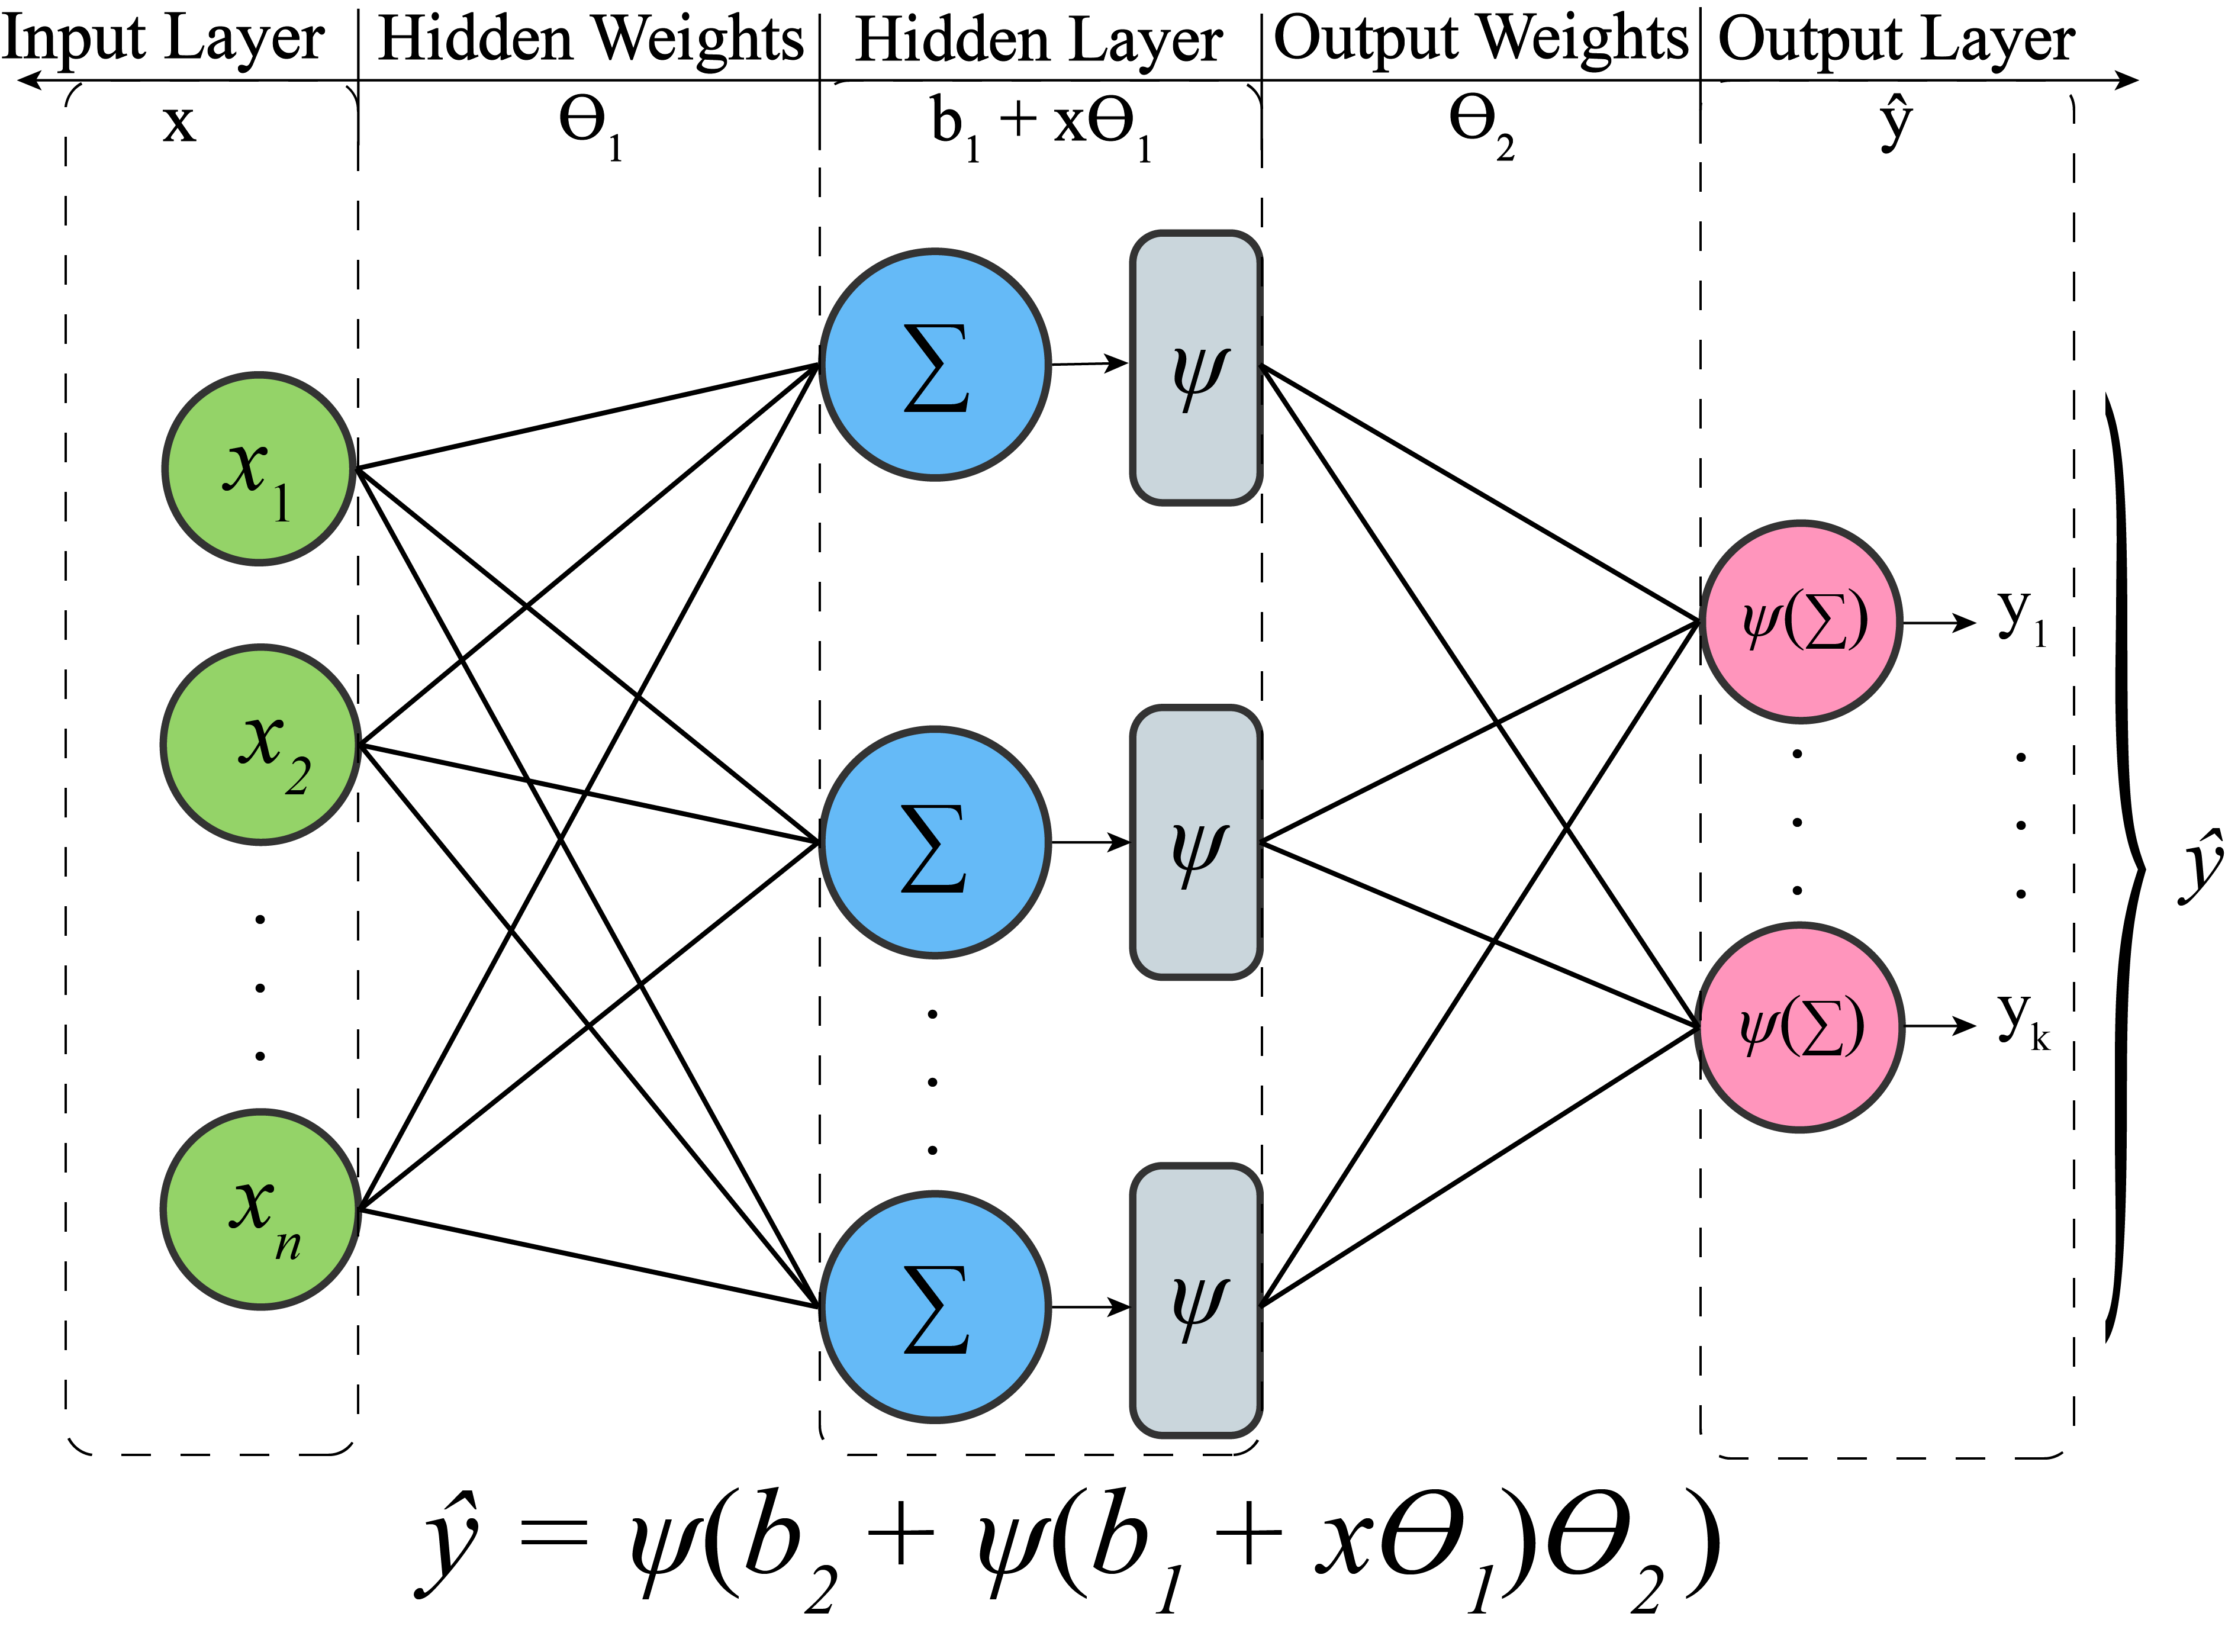
\includegraphics[height = 6cm, width=0.5\textwidth]{img/mlp.png}\label{fig:mlp}}
        %\caption{Feed Forward Multilayer Perceptron}
    \hfill
        \sidesubfloat[]{\includegraphics[height = 6cm, width=0.4\textwidth]{img/actfunc.png}\label{fig:actfunc}}
        %\caption{Common Activation Functions, $\psi$}
        
    \caption{a) Structure of a feed forward MLP with three layers. b) The output for Logistic, Tanh and ReLU activation functions for input value range [-4,4].}\label{fig:mlp_actfunc}
\end{figure}
% Change the italics brackets to regular 
% Add activation function to hidden layer 
%Define supervised classification

A nonlinear activation function $\psi$ allows the compositional output function $ \hat{y}$ to map inputs non-linearly to outputs. Deeper MLPs will contain many more hidden layers then displayed in Fig. \ref{fig:mlp} and a neural network with $n$ layers can be defined recursively as:
\begin{equation}
        \hat{y} = \psi(\theta_{n}(\psi(\theta_{n-1}(\psi(\theta_{n-2}(\ldots \psi(\theta_{1} x + b_{1}) \ldots)) + b_{n-2})) + b_{n-1}) + b_{n}),
\end{equation}

\noindent
,where the structure of $\hat{y}$ depends on the desired task (e.g nonlinear regression or classification). For regression problems, $\hat{y}$ is a real value, and for classification problems, $\hat{y}$ is a $k$ dimensional vector of real values. So although it is generally advantageous for hidden units to have nonlinear activation functions, the choice of activation functions for output layers will largely depend on the desired task. For nonlinear regression, a linear activation function is generally adequate. However, in classification problems, it can be useful to view the $k$ dimensional output vector $\hat{y} = (y_1,y_2,..., y_k)$ as providing the probabilities a given input example resides in each respective class. This produces a probability distribution over the $k$ classes, where entries fall between $(0,1)$, and the sum of the vector $\hat{y}$ is one. This behaviour can be accomplished by the softmax function:
\begin{equation}
       \mathrm{softmax}(z) = \frac{e^{z_j}}{\sum_{i=1}^{k}e^{z_i}} \;\;\; \mbox{for} \;\;\; j = \{1 \ldots k\},
\end{equation}

\noindent
where softmax$(z)$ represents the categorical distribution of arbitrary $k$ dimensional vector $z$. Furthermore, with a formally defined arbitrary output function $\hat{y}$, the next step requires the artificial neural network to learn weights and biases in order to produce desired outputs given input data.

\subsubsection{The Cost Function}
Training an artificial neural network relies on determining the network parameters that minimize the error between outputs $\hat{y}$ and true values $y$. This entails producing a model function, that given inputs, can produce the output to the closest degree. In machine learning, the notion of a good model is explicitly defined using some cost function $J(\hat{y},y;\Theta)$, where $\Theta = \{\theta, b\}$ is the set of all network weights and biases. The cost function keeps track of the model's prediction error. Finding better models equates to finding better network parameters that minimizes the cost function. For nonlinear regression, a commonly used measure of cost is simply the mean squared error between the output of the neural network and the true values:
\begin{equation} \label{eq:mse} 
    J(\hat{y},y;\Theta) = \sum_{i=1}^{m}(y_i - \hat{y_i})^{2}
\end{equation}

For classification problems, it is often beneficial to represent categorical true labels $y$ as binary vectors. This is referred to as one hot encoding, where the $i$th position of class $i$ is one, and every other term is zero. For example, in a five class problem, a class of three would be coded as $y = [0,0,1,0,0]$. In this way, the error must be calculated for each potential class $k$ over all examples in the sample set. Accordingly, the most commonly used cost function for classification problems is the cross entropy loss:
\begin{equation} \label{eq:softmax}
    J(\hat{y}, y; \Theta) = - \frac{1}{m}\sum_{i = 1}^{m}\sum_{j = 1}^{k} \lbrack y_{i,j} \log(\hat{y_{i,j}}) + (1 - y_{i,j})\log(1 - \hat{y_{i,j}}) \rbrack
\end{equation}

In the computation of cross-entropy loss, $k$ error terms are generated for every training example. The cross-entropy loss represents the log probability of classes given the model - that is, maximizing the likely hood of a training example belonging to a specific class is equivalent to minimizing the cross entropy loss between $\hat{y}$ and $y$. 

\subsubsection{The Optimization Algorithm}
The cost, $J(\hat{y}, y; \Theta)$, is conveniently a function of the training examples and model parameters $\Theta$. In order to effectively minimize the cost function, it is useful to observe how the cost changes with respect to weights $\theta$. Formally, this is expressed with the partial derivative $\frac{\partial J}{\partial \theta}$. With this expression, we can search for weights in the direction that cost $J$ decreases. This technique, called gradient descent, minimize cost by iteratively updating $\theta$ in the opposite direction of the gradient:

\begin{equation}\label{eq:update}
    \theta_j = \theta_j - \alpha \frac{\partial}{\partial \theta_j} J(\hat{y},y;\Theta) \;\;\; \mbox{for} \;\;\; j = \{1,\ldots,n\},
\end{equation}

\noindent
where $\alpha$, the learning rate, controls the size of steps made in the direction of the negative gradient. Furthermore, in order to compute the gradients of the cost with respect to model weights, an algorithm called backpropagation is commonly used. The cost function, as one large nested composite function, contains all of the computations in the neural network. With this, the backpropagation algorithm cleverly applies the chain rule of calculus to recursively compute the gradients of each weight, as shown in Fig. \ref{fig:backprop}. 

%with respect to the outputs so weights can be updated incrementally using gradient descent. 

\begin{figure}[htb]
    \centering
    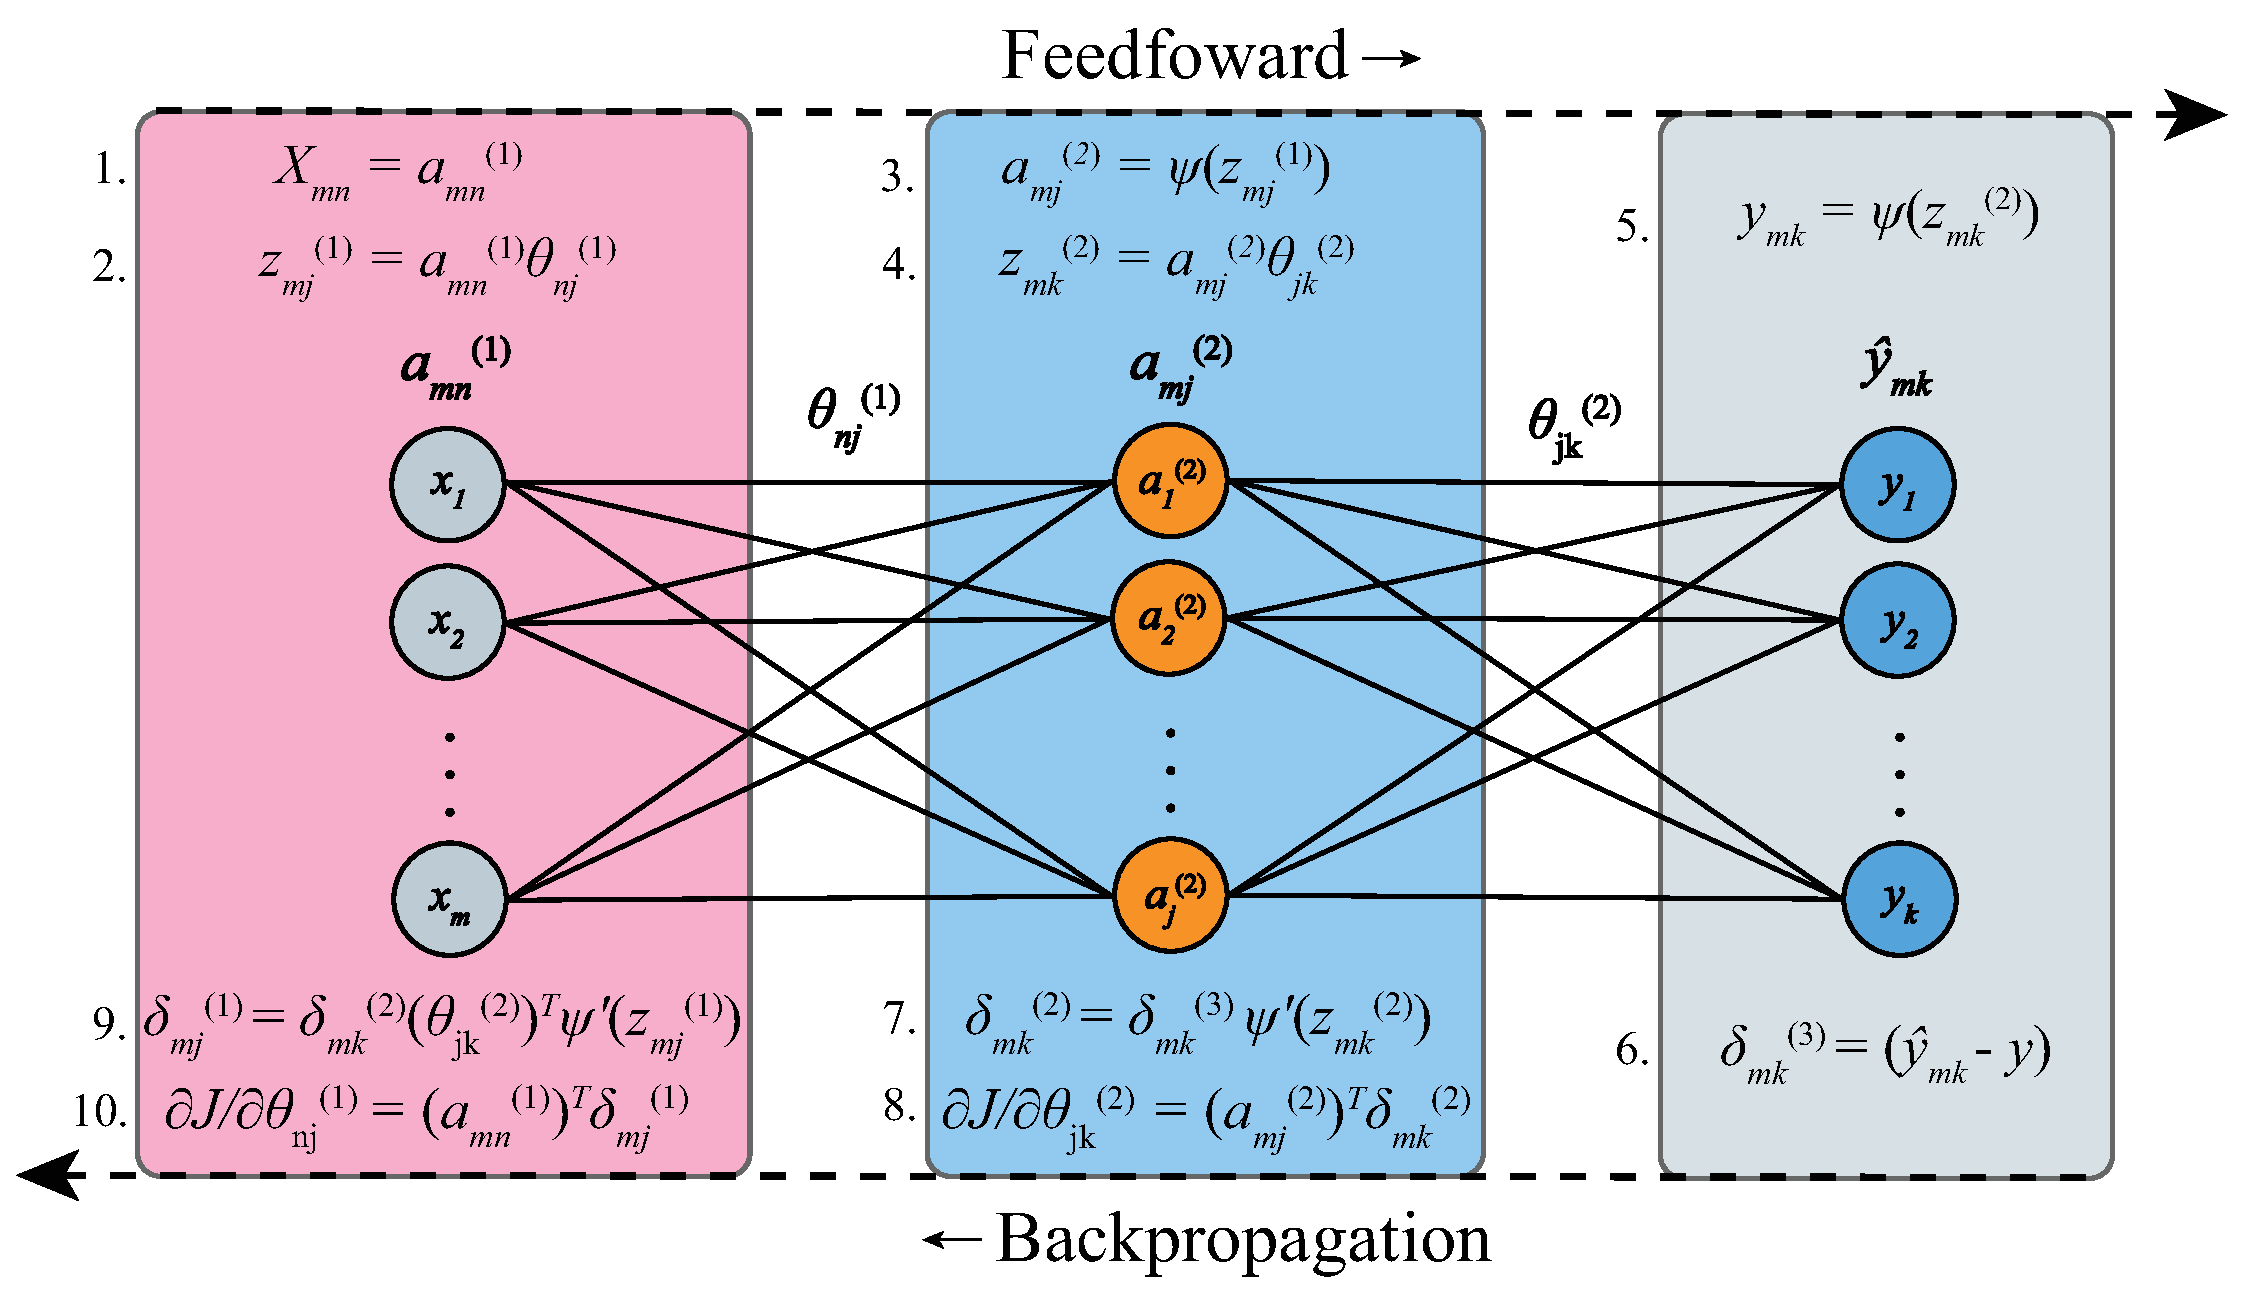
\includegraphics[width=\textwidth]{img/backprop.eps}
    \caption{Feedforward and Backpropagation Schematic.}
    \label{fig:backprop}
\end{figure}

Fig. \ref{fig:backprop} illustrates the mechanism of a feedforward multilayer perceptron with an input layer $X_{mn}$, a hidden layer $a_{mj}^{(2)}$, and an output layer $\hat{y}_{mk}$. The input layer, considered the first activation $a_{mn}^{(1)}$, is used to form the first linear combination $z_{mf}^{(1)}$. In the hidden layer, a nonlinear activation function $\psiup(z_{mj}^{(1)})$ is used to produce the hidden activations $a_{mj}^{(2)}$. In deeper networks, the preceding layers outputs are continually utilized in a series of linear combinations, following by nonlinear activation functions until the output layer is reached. At this point, the model predictions are compared to the true values using cost function $J(\hat{y}_{mk})$. In order to train the neural network, or minimize the cost function, the gradient of the cost function is computed to determine the direction in the parameter space required to lower network error. The gradient of the cost function is computed efficiently propagating the error back through the network using the derivate chain rule. In Fig. \ref{fig:backprop}, backpropagation begins with the output \textit{backpropagation-error} $\delta_{mk}^{(3)} = (\hat{y_{mk}} - y_{mk})$ shown in step 10. \textit{Backpropagation-error} is the layer specific approximation error, and the hidden and input layer \textit{backpropagation-errors} are represented as $\delta_{mk}^{(2)}$ and $\delta_{mf}^{(1)}$, respectively. In Eq. \ref{eq:update}, we see that the partial derivative of the cost function with respect to each weight is required in order to compute a gradient update. In this example, the weights of the model are spread across two matrices, $\theta_{nf}^{(1)}$ and $\theta_{jk}^{(2)}$. Accordingly, we will calculate gradient matrices of the same dimension, $\partial J / \partial \theta_{nf}^{(1)}$ and $\partial J / \partial \theta_{jk}^{(2)}$, to store the gradient of the cost function with respect to each weight in the model. Starting with $\partial J / \partial \theta_{jk}^{(2)}$, we get the following expression using squared error as the cost function:

\begin{equation*}
    \frac{\partial J}{\partial \theta_{jk}^{(2)}} =  \frac{\partial \frac{1}{2}\sum (y_{mk} - \hat{y}_{mk})^{2}}{\partial \theta_{jk}^{(2)}}
\end{equation*}

\noindent
If we remove the summation from this expression we can compute the gradient for a single example. Evaluating the resultant derivative produces:

\begin{equation*}
    \frac{\partial J}{\partial \theta_{jk}^{(2)}} =  -(y_{mk} - \hat{y}_{mk})\frac{\partial \hat{y}_{mk}}{\partial \theta_{jk}^{(2)}}\\
\end{equation*}

\noindent
From step 5 on Fig. \ref{fig:backprop}, we see that $\hat{y}_{mk} = \psiup(z_{mk}^{(2)})$. Accordingly, we can now apply the chain rule to further evaluate the expression: 

\begin{equation*}
    \frac{\partial J}{\partial \theta_{jk}^{(2)}} =  -(y_{mk} - \hat{y}_{mk}) \frac{\partial \hat{y}_{mk}}{\partial z_{mk}^{(2)}} \frac{\partial z_{mk}^{(2)}}{\partial \theta_{jk}^{(2)}}\\
\end{equation*}

\noindent
We can now replace $\partial \hat{y}_{mk} / \partial z_{mk}^{(2)}$ with $z_{mk}^{(2)}$ evaluated by the derivative of the activation function, $\psiup'(z_{mk}^{(2)})$. As well, from step 4 on Fig. \ref{fig:backprop}, we see that $z_{mk} = a_{mj}^{(2)}\theta_{jk}^{(2)}$. The derivative of this linear relationship is simply the slope $a_{mj}^{(2)}$. We can now simplify our expression:

\begin{equation*}
    \frac{\partial J}{\partial \theta_{jk}^{(2)}} =  -(y_{mk} - \hat{y}_{mk}) \psiup'(z_{mk}^{(2)}) a_{mj}^{(2)}
\end{equation*}

\noindent
The hidden layer \textit{backpropagation-error} is given by $\delta_{mk}^{(2)} = -(y_{mk} - \hat{y}_{mk})\psiup'(z_{mk}^{(2)})$. Notice that if we transpose the activity matrix $a_{mj}^{(2)}$, we can perform matrix multiplication with $a_{mj}^{(2)}$ and $\delta_{mk}^{(2)}$ to sum across all examples. This effectively takes care of the earlier omission of the summation, so that the gradient can be calculated efficiently as shown in step 8 on Fig. \ref{fig:backprop}. The simplified expressions becomes:

\begin{equation*}
    \frac{\partial J}{\partial \theta_{jk}^{(2)}} =  (a_{mj}^{2})^{T}\delta_{mk}^{(2)}
\end{equation*}

\noindent
The derivation for $\partial J / \partial \theta_{nj}^{(1)}$ begins the same way as described above, but diverges when the chain rule is used to expand $\partial z_{mk}^{(2)}/\partial \theta_{nj}^{(1)}$:
 
\begin{equation*}
\begin{split}
\frac{\partial J}{\partial \theta_{nj}^{(1)}} & = \delta_{mk}^{(2)} \; \frac{\partial z_{mk}^{(2)}}{\partial \theta_{nj}^{(1)}} \\
 & = \delta_{mk}^{(2)} \; \frac{\partial z_{mk}^{(2)}}{\partial a_{mj}^{(2)}} \; \frac{\partial a_{mj}^{(2)}}{\partial \theta_{nj}^{(1)}}\\
& = \delta_{mk}^{(2)} \; (\theta_{jk}^{(2)})^{T} \; \frac{\partial a_{mj}^{(2)}}{\partial \theta_{nj}^{(1)}}\\
& = \delta_{mk}^{(2)} \; (\theta_{jk}^{(2)})^{T} \; \frac{\partial a_{mj}^{(2)}}{\partial z_{mf}^{(1)}} \; \frac{\partial z_{mf}^{(1)}}{\partial \theta_{nj}^{(1)}}\\
& = \delta_{mk}^{(2)} \; (\theta_{jk}^{(2)})^{T} \; \psiup'(z_{mf}^{(1)}) \; \frac{\partial z_{mf}^{(1)}}{\partial \theta_{nj}^{(1)}}\\
& = (a_{mn}^{(1)})^{T} \; \delta_{mk}^{(2)} \; (\theta_{jk}^{(2)})^{T} \; \psiup'(z_{mf}^{(1)})\\
& = (a_{mn}^{(1)})^{T} \; \delta_{mj}^{(1)}
\end{split}
\end{equation*}

\noindent
The simplified expression for both gradients are closely related. We see that the gradients depend on the layer activity and the \textit{backpropagation-error}. In turn, the calculations for \textit{backpropagation-error} are dependent on the error terms in the next layer. Thus, computation of error proceeds backwards from the output layer towards the input layer. This is where backpropagation, or backwards propagation of errors, gets its name. The error $\delta^{\ell}$ at layer $\ell$ is dependent on the errors $\delta^{\ell+1}$ at the next layer $\ell + 1$. 

%In Figure \ref{fig:actfunc}, we see that the tanh and logistic functions have sigmoidal shapes, mapping all inputs between $(-1,1)$ and $(0,1)$, respectively. In the output layer, this kind of behaviour makes them useful for classification problems. Though for nonlinear regression, a linear output activation would be beneficial. Accordingly, the choice of activation functions will largely depend on the desired task, but it is generally desired for the hidden units to have nonlinear activation functions. Deeper MLPs will contain many more hidden layers then displayed in Figure \ref{fig:mlp}, 

%%The cost function, as one large nested composite function, contains all of the computations in the neural network. 

\section{Deep Learning} \label{sec:deeplearning}

\subsection{Deep Neural Networks}

%Explain what deep learning is, why it is used (representation learning)

Deep learning is a subset of machine learning based on artificial neural networks. Deep learning employs architectures such a deep neural networks (DNN) that typically have multiple layers between the input and the output layers. DNNs learn hierarchical representations of the data through the layers of the network in order to map complex relationships between the input and the desired outputs. Recently, these networks have made state-of-the-art breakthroughs in fields such as natural language processing, computer vision, and speech recognition.

DNNs are especially useful for learning intermediate representations of input data. The representations are formed with the composition of non-linear transformations through multiple layers in the network. The output of each layer forms a hierarchy of distributed representations that have an increasing level of abstraction as an input flows through the network. The performance of a DNN depends largely on the representations it learns to output. This is because the distribution of the input data is generated by a combination of underlying features and a model that learns to compactly represent the features can generalize for more variation without requiring as many examples. In cases where the transformation results in data compression the learning task equates to developing output representations that map to the naturally occurring input data distribution but in a low dimensional manifold.

\subsection{Autoencoders}

Autoencoders represent a family of unsupervised artificial neural networks that learn latent data codings for input data. Here, training examples are utilized without labels, and autoencoders are trained to generate outputs identical to the inputs. The role of an autoencoder is split into two tasks, encoding and decoding. The process of encoding maps the input to lower dimension features, and decoding maps the encoded data back into the original space. The mapping of an input layer produced by function, $g_{\theta}(\cdot)$, can be expressed as:
 
\begin{equation}
z = g_{\theta}(x) = \psi(\theta x + b)
\end{equation}

This latent layer, of potentially reduced dimensionality, can then be decoded back to the original space with function $f_{\theta^{T}}(\cdot)$:

\begin{equation}
x' = f_{\theta^{T}}(z) =  f_{\theta^{T}}(g_{\theta}(x)) = (\theta^{T}z + b)
\end{equation}

Where $x'$ is the reconstructed input data, and $\theta^{T}$ is the transpose of weights used for encoding. Furthermore, to train the model, the reconstructed output is compared to the original input using the mean squared error to calculate reconstruction error:

\begin{equation}
J(x'_{i},x_{i};\Theta) = \frac{1}{2m}{\sum^{m}_{i=1}} ||x_i - x'_i||^2
\end{equation}

Where $\Theta = \{\theta, b_\theta,\theta^{T}, b_{\theta^{T}}\}$ is the set of network parameters used for encoding and decoding operations. 

\subsubsection{Denoising Autoencoders}
Training an autoencoder with partially corrupted data while comparing the reconstruction to the original input is a commonly used technique to increase the robustness of an autoencoder. This modification produces a variant of the basic autoencoder called a denoising autoencoder. By adding corruption to the input data, $\tilde{x}_{i} \sim \mu_{D}(\tilde{x}_{i}|x_{i})$, the autoencoder must learn parameters that can overcome stochastic noise. The operation $\mu_{D}$ defines the form of noise used to corrupt the input data in order to increase robustness, and the reconstruction error is calculated using cost $J(\tilde{x}'_{i},x_{i};\Theta)$. 

Furthermore, deeper frameworks of denoising autoencoders, called stacked denoising autoencoders (SDAEs), are employed to increase the number of latent abstractions. SDAEs are composed of multiple layers of incrementally stacked denoising autoencoders that are trained one layer at a time \cite{vincent2010stacked}. In this way, once the $k$th hidden layer is trained, layer $k+1$ can be trained using the $k$th layer as the input data.

% Add figures for stacked denoising autoencoder

\section{Improving Machine Learning Models}

\subsection{Regularization}
%Talk about overfitting
%Regularization

A key aspect of producing a good machine learning model is to avoid overfitting the training data. The problem of overfitting arises when the model variables and parameters aggressively captures both the underlying pattern and stochastic noise of the training data. The model is learning information that does not represent the true properties of the underlying relationship when it captures too much random noise. In this case, the model will perform well on the test set, but will likely have a poor prediction and generalization power on examples it has never seen before. 

This problem gets worst as the model complexity increases, and the model variables and paramaters have the flexibility to increasingly capture background noise. A way to avoid overfitting is by using cross validation. Cross validation is beneficial because the model variables and parameters are decided by estimating the error of the model over a subset of the data the model has not observed. In $k$-fold cross validation, this is performed by dividing the data into $k$ subsets. Then each of the $k$ subsets are used as a validation set, and the other $k-1$ subsets are combined as the training set. Accordingly, the error estimation gets averaged over the $k$ trials to compute the total effectiveness of the model.

Furthermore, another commonly used way to avoid overfitting is through model regularization. Regularization is a form of regression that applies a constraint to the model complexity. Ridge regression involves penalizing the cost function during the training procedure by adding a multiple of the squared magnitude of the model coefficients. Accordingly, ridge regression employs weighted L2 regularization producing the following loss equation:

\begin{equation} \label{eq:l2reg}
    \mathrm{Loss} = J(\hat{y},y;\Theta) + \frac{\lambda}{2m} \sum_{j=1}^{m} \sum_{k=1}^{p} \Theta_{j,k}^{2} \;\;,
\end{equation}

\noindent
where m is the number of training examples, p is the number of model weights, and $\lambda$ is the regularization parameter. Here, $\lambda$ decides how much the model flexibility should be penalized. When $\lambda = 0$, the penalty term is ignored, and the trained model is susectible to overfitting. However, as $\lambda \rightarrow \infty$, the model weights are increasingly penalized and will approach zero. This will result in under-fitting, where the model losses the ability to fit the data entirely. Therefore, selecting a good regularization parameter is essential for optimizing the performance of the machine learning model. 


\subsection{Model Averaging}
%Model Averaging - dropout and maxout model

The dropout technique is a relatively simple way to regularize a neural network using the concept of model averaging. Dropout entails randomly setting a fraction of the neurons in the network to zero during forward propagation. At each training step, a neuron is either kept with a probability of $p$, or \textit{dropped out} with probability $1-p$ to produce a network of reduced size. During backpropagation, the weights of dropped out neurons will not be updated. Accordingly, dropout is training a subsample of the whole neural network on every training iteration. In this way, dropout can be seen as an ensemble of randomly sampled models that share parameters. As well, dropout is a useful technique for addressing co-adapting behaviour in machine learning models. Co-adaptation occurs when neurons learn to fix the mistakes of other neurons in a fully connected neural network. This is a problem because co-adapted neurons tend to result in overfitting because they do not generalize well to new data. With dropout, neurons are forced to learn more robust features that are independent to the other neurons. 

\begin{figure}[htb]
    \centering
        \sidesubfloat[]{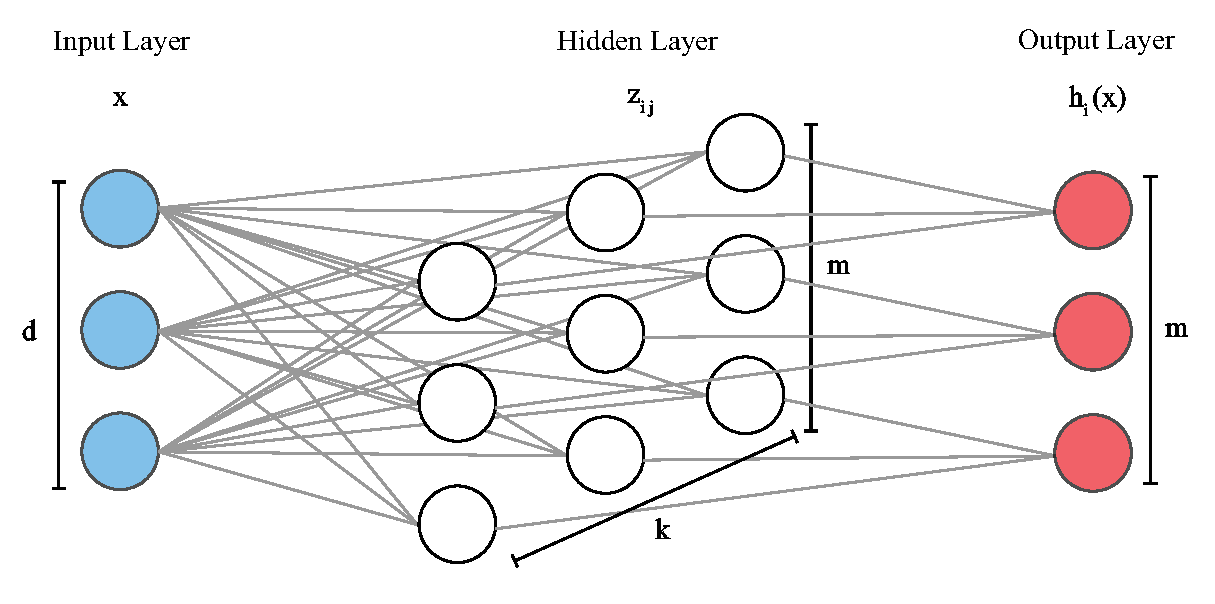
\includegraphics[width=0.7\textwidth]{img/maxout1.eps}\label{fig:maxout_a}}
        %\caption{Feed Forward Multilayer Perceptron}
    \hfill
        \sidesubfloat[]{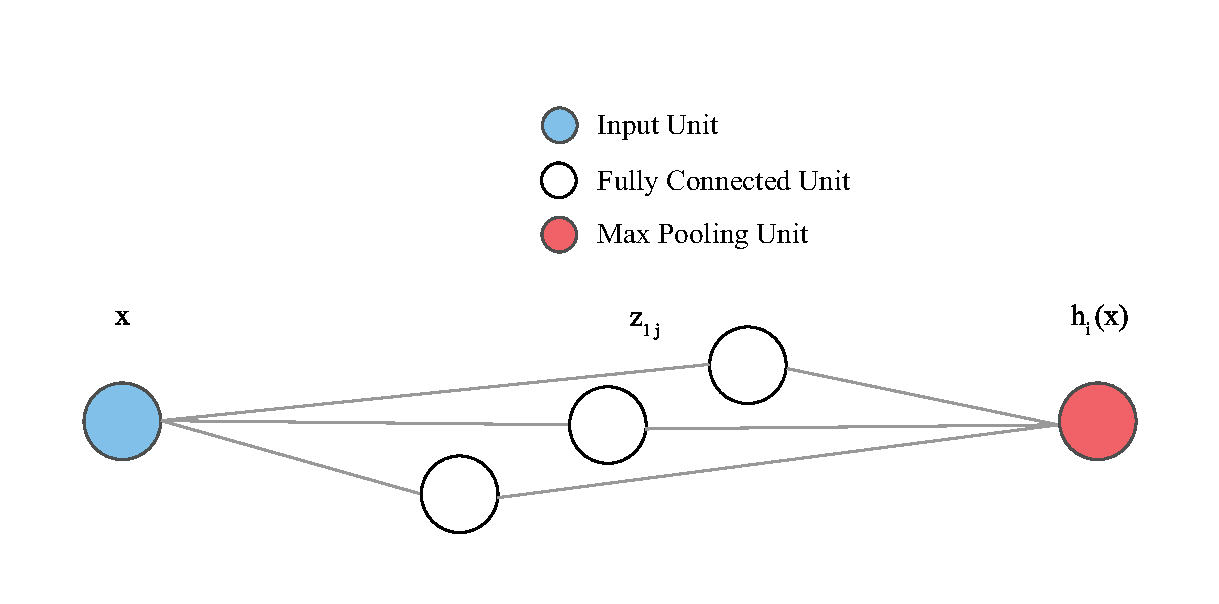
\includegraphics[width=0.7\textwidth]{img/maxout2.eps}\label{fig:maxout_b}}
        %\caption{Common Activation Functions, $\psi$}
        
    \caption{a) Structure of a maxout neural network b) Maxout neural network with d = 1, m = 1, and k =3}\label{fig:maxout}
\end{figure}

Furthermore, an activation function called maxout was proposed to leverage the model averaging performed by dropout \cite{goodfellow2013maxout}. The maxout activation function was shown to improve approximate model averaging in deep models over non-linear activations such as the Tanh function \cite{goodfellow2013maxout}. Formally, the maxout activation function is defined as: 

\begin{equation} \label{eq:maxout}
    h_{i}(x) = \underset{j \in [1,k]}{\mathrm{max}}z_{i,j},
\end{equation}

\noindent
where $x \in \mathbb{R}^{n}$ is an input vector, $z_{i,j} = x^{T}W_{...ij}v + b_{ij}$ is output for the $j$-th linear transformation of the $i$-th hidden unit, and $W \in \mathbb{R}^{d \times m \times k}$ and $b \in \mathbb{R}^{m \times k}$ are learned parameters. In simple terms, maxout accepts an input of dimensionality $d$ and computes $k$ linear transformations and returns the largest unit for each of the $m$ linear feature extractors. The maxout activation function is applied by using a small differentiable sub-network as shown in Fig. \ref{fig:maxout}.

\begin{figure}[ht]
    \centering
    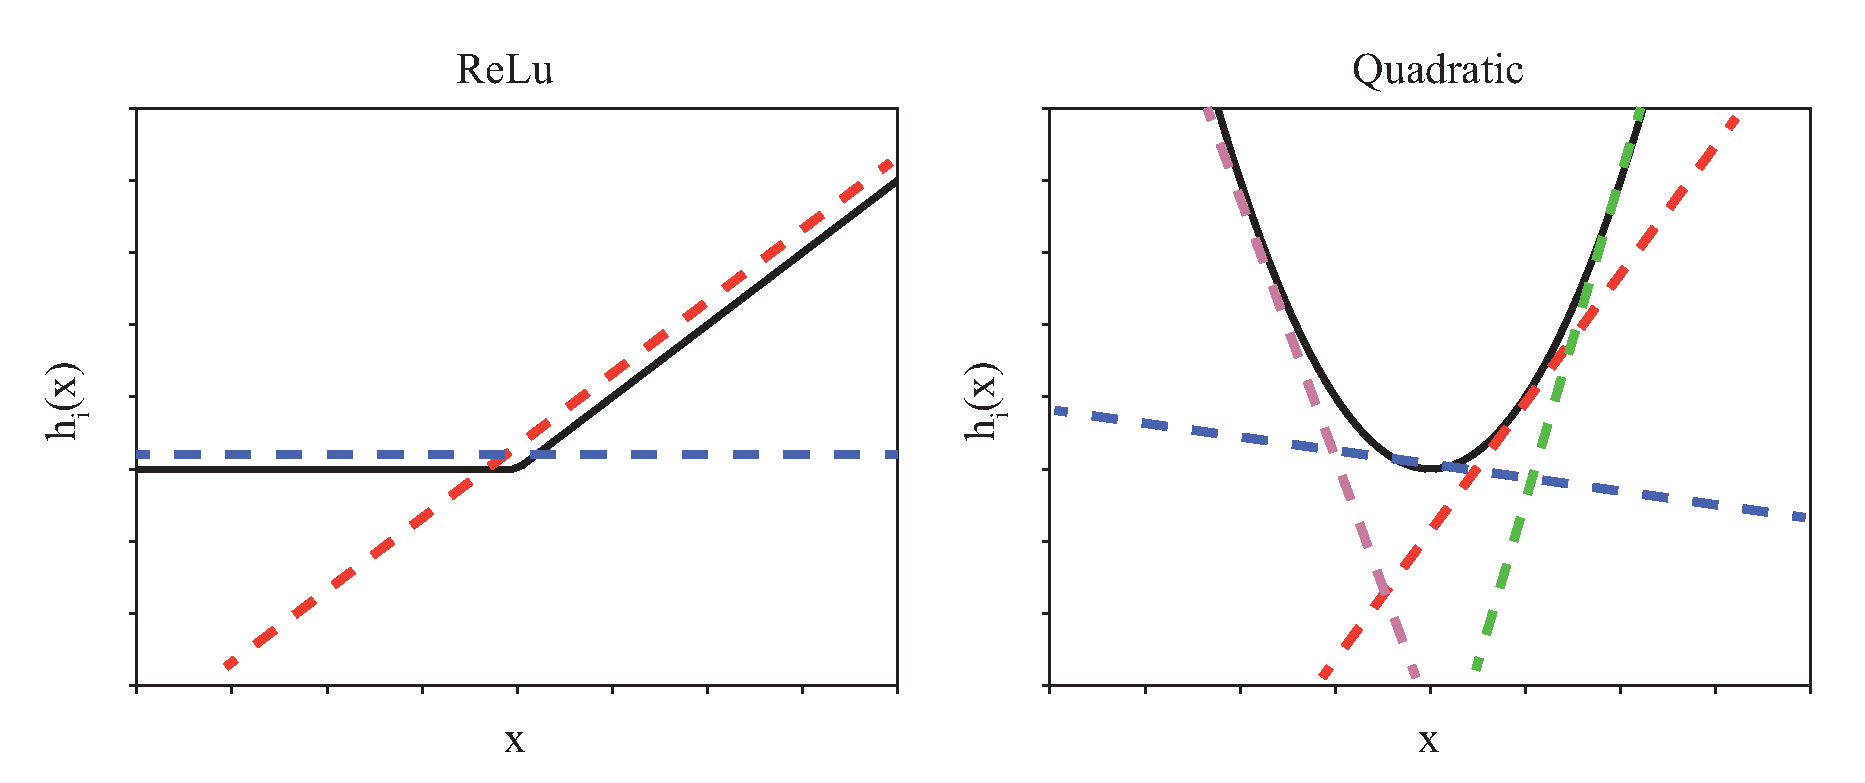
\includegraphics[width=0.7\textwidth]{img/max_func.eps}
    \caption{Maxout approximation of ReLu and quadratic activation functions.}
    \label{fig:maxout_func}
\end{figure}

In Fig. \ref{fig:maxout_a}, the hidden layer implements the weighted sum of all inputs. In Eq. \ref{eq:maxout}, this is represented by $z_{i,j} = x^{T}W_{...ij} + b_{ij}$. The three-dimensional tensor $W_{...ij}$, represents the weight vector for the unit in row $i$ and column $j$ of the fully connected units. The max pooling units simply take the maximum output from the neurons of each row. From Fig. \ref{fig:maxout_func}, we can see how the maxout activation function can approximate a ReLu and qaudratic activation function. In this way maxout can produce a piecewise linear approximation of an arbitrary convex function.